\documentclass[12pt]{article}

\usepackage[utf8]{inputenc}
\usepackage[english,russian]{babel}
\usepackage{amsmath, amssymb}
\usepackage{graphicx}
\usepackage{epstopdf}
\usepackage{algorithm}
\usepackage{algpseudocode}

\newcommand{\cutefrac}[2]{{}^{#1\!}\!/{\!}_#2}
\newcommand{\half}{\cutefrac{1}{2}}
\newcommand{\cuteddots}{
\text{
\raisebox{.6ex}{$\cdot$}\hspace{.75em}%
\raisebox{.3ex}{$\cdot$}\hspace{.75em}%
$\cdot$\hspace{.75em}%
\raisebox{-.3ex}{$\cdot$}\hspace{.75em}%
\raisebox{-.6ex}{$\cdot$}%
}}

\graphicspath{{mp/}}

\title{Задание 3}
\date{}

\begin{document}

\maketitle

Для задачи 
\begin{equation}
\begin{cases}
-\omega^2 u = c^2(x) u_{xx}\\
u(0) = 1\\
i\omega u(1) + c(1) u_x(1) = 0
\end{cases},
\label{eq:stationary}
\end{equation}
полученной из волнового уравнения подстановкой $p(t,x) =
\operatorname{Im}\left[e^{i\omega t} u(x)\right]$ граничное условие на правой
границе означало условие выхода волн за пределы области без отражений.

Для более сложных задач такой подход уже не работает. Для решения проблемы
постановки прозрачных (вернее, поглощающих) условий был разработан PML. PML
расшифровывается как perfectly matching layer или идеально согласованный слой.
Суть метода в том, что расчетная область увеличивается, и в добавленном участке
решается исходное уравнение, но исправленное так, чтобы волны, попадающие в него
быстро затухали. При этом граничные условия (которые теперь ставятся на границе
PML области, а не расчетной области) могут быть произвольными.

Добавим к отрезку $[0, 1]$, который мы рассматривали ранее, поглощающий слой на
отрезке $[1, 2]$. Необходимо понять, как нужно модифицировать уравнение на $[1,
2]$, чтобы волны в этой среде затухали.

\section{Основы PML}

Рассмотрим волновое уравнение
\[
p_{tt} = c^2(x) p_{xx},\quad x \in \mathbb{R}
\]
где $p(t, x)$ --- аналитическая по $x$ в каждый момент времени $t$ функция. 
Эту функцию можно рассматривать как <<срез>> решения уравнения
\[
P_{tt} = c^2(z) P_{zz},\quad z \in \mathbb{C}
\]
на линии $z = x + 0i$: $p(t, x) = P(t, x + 0i)$. 
Фактически, задавая разные линии в плоскости $\mathbb{C}$ мы будем получать
разные срезы одной и той же функции $P(t, z)$. 
Рассмотрим изображенную на следующем рисунке линию в комплексной плоскости:
\begin{figure}[ht!]
\centering
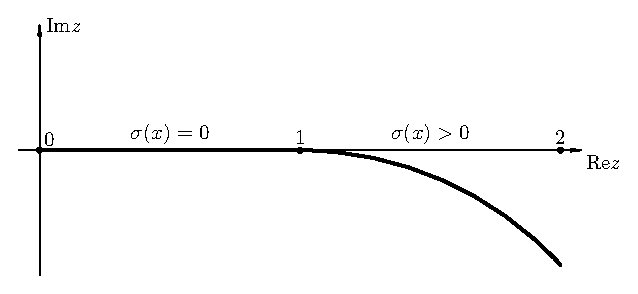
\includegraphics[width=.8\textwidth]{func-0.eps}
\caption{Вид линии $z(x)$, используемый для одномерного PML}
\end{figure}

Она параметризована следующим образом:
\[
z(x) = \int_0^x 1 - \frac{i}{\omega}\sigma(\xi) d\xi = x - \frac{i}{\omega} \int_0^x \sigma(\xi) d\xi
\]
Там, где $\int_0^x\sigma(\xi)d\xi = 0$ линия не отличается от отрезка
действительной оси, на нем решение $P(t, z)$ имеет вид решения волнового уравнения $p(t,
x)$.

На линии $z(x)$ мы можем получить из уравнения для $P(t, z)$ уравнение для $p(t,
x) = P(t, z(x))$. Для этого нужно сделать замену переменных 
\[
\frac{\partial}{\partial z} = \frac{d x}{d z} \frac{\partial }{\partial x} = 
\frac{1}{dz/dx} \frac{\partial}{\partial x} = 
\frac{\omega}{\omega - i\sigma(x)} \frac{\partial}{\partial x}.
\]
Смысл $\omega$ в этой формуле в том, что конкретная замена координат оказывается
разной для разных Фурье-компонент решения. В нашей стационарной задаче
фиксировано стационарное решение, состоящее всего из одной компоненты
$e^{i\omega t}u(x)$, поэтому $\omega$ в этой формуле --- просто константа.

Производя эту замену в уравнении $P_{tt} = c(z)^2 P_{xx}$, получаем уравнение
следующего вида:
\begin{gather*}
P_{tt} = c^2(z(x)) 
\frac{\omega}{\omega - i\sigma(x)} 
\frac{\partial}{\partial x}
\left(
\frac{\omega}{\omega - i\sigma(x)} 
\frac{\partial P}{\partial x}
\right)
\end{gather*}

Чтобы понять, как влияет такая замена координат, рассмотрим задачу с постоянными
коэффициентами:
\[
u_{tt} = c^2 \frac{\omega^2}{(\omega - i\sigma)^2} u_{xx}
\]
Рассмотрим преобразование Фурье по времени от этого уравнения, $\hat u =
\mathcal{F}[u]$:
\[
-\omega^2 \hat u = c^2 \frac{\omega^2}{(\omega - i\sigma)^2} \hat{u}_{xx}
\]
Каждая волна вида $\hat u = e^{ikx}$ будет решением этого уравнения при
\[
(\omega - i\sigma)^2 = (ck)^2 \qquad \omega = i\sigma \pm ck
\]
Решение $u$ будет состоять из суперпозиции затухающих волн:
\[
\exp\left\{-\sigma t + ik(x \pm ct)\right\}
\]
Поскольку все составляющие решения затухают, и все решение будет затухать во
времени.

К сожалению, зависимость преобразования координат от частоты --- необходимость.
Например, простым преобразованием
\[
\frac{\partial}{\partial z} = 
\frac{1}{1 - i\sigma(x)} \frac{\partial}{\partial x}.
\]
обойтись не получается, так как аналогичные рассуждения приводят нас к следующей
связи между $\omega$ и $k$:
\[
-\omega^2 \hat u = c^2 \frac{-k^2}{1 - i\sigma} \hat u \qquad \omega = \pm
\frac{ck}{\sqrt{1 - i\sigma}} = \pm ck(\alpha + i\beta)
\]
При этом, одно из решений 
\[
\exp\left\{\mp ck\beta t + ik(x \pm ct\alpha)\right\}
\]
во времени уменьшается, а второе --- растет.

\section{Конкретная задача}

Поскольку нас интересует стационарная компонента $P = e^{i\omega t}
u(x)$, рассмотрим следующее уравнение:
\begin{equation}
-\omega^2 u(x) = 
c^2(z(x)) 
\frac{\omega}{\omega - i\sigma(x)} 
\frac{\partial}{\partial x}
\left(
\frac{\omega}{\omega - i\sigma(x)} 
\frac{\partial u}{\partial x}
\right)
\label{eq:problem}
\end{equation}

Здесь $\omega$ --- просто числовая константа. Заметим, что в уравнение входит
скорость звука, взятая на линии $z = x + i \int_0^x \sigma(\xi) d\xi$. Значение
$c(z)$ получается из функции $c(x)$ её аналитическим продолжением. При этом,
скорость звука вдоль линии $z(x)$ вполне может стать комплексной, что не
желательно. Поэтому, в области $x > 1$, где находится PML слой, скорость
необходимо положить равной константе $c(x) = c(1), x > 1$. При этом ее
аналитическое продолжение также будет константой $c(1)$. Теперь можно в
уравнении \eqref{eq:problem} заменить $c(z(x))$ на $c(x)$, поскольку они
совпадают как в области решения, так и в PML области.
\begin{equation}
-\omega^2 u(x) = 
c^2(x) 
\frac{\omega}{\omega - i\sigma(x)} 
\frac{\partial}{\partial x}
\left(
\frac{\omega}{\omega - i\sigma(x)} 
\frac{\partial u}{\partial x}
\right)
\label{eq:problem2}
\end{equation}

Применим ту же технику интегрирования с весом $w(x)$, что и раньше,
предварительно перенеся множитель перед $\frac{\partial}{\partial x}$ налево:
\begin{gather}
-\omega^2 \frac{\omega - i\sigma(x)}{\omega} u(x) - \frac{\partial}{\partial x} 
\left(
\frac{\omega}{\omega -i\sigma(x)} \frac{\partial u}{\partial x}
\right) = 0\\
-\omega^2 \int_0^2 \frac{\omega - i\sigma(x)}{\omega} u(x) w(x) dx 
-\frac{\omega}{\omega -i\sigma(x)} u'(x) w(x) \Big|_0^2 
+ \nonumber\\ + \int_0^2 \frac{\omega}{\omega -i\sigma(x)} u'(x) w'(x) dx = 0 
\label{eq:weak}
\end{gather}

Условие $u(0) = 1$ налагает ограничение на $w(x)$: $w(0) = 0$. В точке $x = 1$
положим $u'(2) = 0$. Поскольку PML поглощает все волны, условие на правой
границе не существенно, ослабленные отраженные волны снова будут вынуждены 
пройти поглощающий слой (как мы видели выше, PML поглощает как волны с $k > 0$,
так и $k< 0$ с одинаковым коэффициентом затухания).

Как следует из граничных условий, выражение $u'(x)w(x)$ обращается в ноль как в
точке $x = 0$, так и в $x = 2$. В уравнении \eqref{eq:weak} остается только
\[
-\omega^2 \int_0^2 \frac{\omega - i\sigma(x)}{\omega c^2(x)} u(x) w(x) dx 
+\int_0^2 \frac{\omega}{\omega -i\sigma(x)} u'(x) w'(x) dx = 0 
\]
Подставляя, как это уже делалось раньше,
\[
u(x) = \sum_{k=0}^N u_k \psi_k(x) \qquad w(x) = \psi_j(x), j = 1, 2, \dots, N,
\]
получаем систему линейных уравнений
\begin{equation}
\sum_{k = 0}^N u_k (-\omega^2 M_{kj} + K_{kj}) = 0, \quad j = 1, 2, \dots, N.
\label{eq:system}
\end{equation}
Здесь введены обозначения
\[
M_{kj} = \int_0^2 \frac{\omega - i\sigma(x)}{\omega c^2(x)} \psi_i(x) \psi_j(x) dx
\qquad
K_{kj} = \int_0^2 \frac{\omega}{\omega -i\sigma(x)} \psi_k'(x) \psi_j'(x) dx
\]
Для краткости обозначим дополнительно
\[
\gamma(x) = \frac{\omega - i\sigma(x)}{\omega c^2(x)}
\qquad 
\kappa(x) = \frac{\omega}{\omega - i\sigma(x)}.
\]
Матрицы при этом записываются в виде
\begin{gather*}
M = \frac{h}{6}
\begin{pmatrix}
2\gamma_{\half} & \gamma_{\half} & \\
\gamma_{\half} & 2\gamma_{\half} + 2\gamma_{\cutefrac{3}{2}} & \gamma_{\cutefrac{3}{2}}\\
& \gamma_{\cutefrac{3}{2}} & 2\gamma_{\cutefrac{3}{2}} + 2\gamma_{\cutefrac{5}{2}} & \gamma_{\cutefrac{5}{2}}\\
& & \cuteddots\; & \cuteddots & \;\cuteddots \\
& & & \gamma_{N - \cutefrac{3}{2}} & 2\gamma_{N - \cutefrac{3}{2}} + 2\gamma_{N
- \half} & \gamma_{N-\half}\\
& & & & \gamma_{N - \half} & 2\gamma_{N-\half}
\end{pmatrix}
\\
K = \frac{1}{h}
\begin{pmatrix}
\kappa_{\half} & -\kappa_{\half} & \\
-\kappa_{\half} & \kappa_{\half} + \kappa_{\cutefrac{3}{2}} & -\kappa_{\cutefrac{3}{2}}\\
& -\kappa_{\cutefrac{3}{2}} & \kappa_{\cutefrac{3}{2}} + \kappa_{\cutefrac{5}{2}}
& -\kappa_{\cutefrac{5}{2}}\\
& & \cuteddots\; & \cuteddots & \;\cuteddots \\
& & & -\kappa_{N - \cutefrac{3}{2}} & \kappa_{N - \cutefrac{3}{2}} + \kappa_{N
- \half} & -\kappa_{N-\half}\\
& & & & -\kappa_{N - \half} & \kappa_{N-\half}
\end{pmatrix}
\end{gather*}
Исключаем из системы известную $u_0 = 1$, получая систему для $u_1, \dots, u_N$:
\[
\sum_{k = 1}^N u_k (-\omega^2 M_{kj} + K_{kj}) = \omega^2 M_{0j} - K_{0j} \equiv
f_j, \qquad j = 1, 2, \dots, N.
\]
Окончательно, запишем систему в матричном виде
\begin{equation}
(-\omega^2 \mathbf{M} + \mathbf{K})\mathbf{u} = \mathbf{f},
\label{eq:final}
\end{equation}
где $\mathbf{M}$ и $\mathbf{K}$ получаются из $M$ и $K$ вычеркиванием нулевой
строки и столбца
\begin{gather*}
\mathbf{M} = \frac{h}{6}
\begin{pmatrix}
2\gamma_{\half} + 2\gamma_{\cutefrac{3}{2}} & \gamma_{\cutefrac{3}{2}}\\
\gamma_{\cutefrac{3}{2}} & 2\gamma_{\cutefrac{3}{2}} + 2\gamma_{\cutefrac{5}{2}} & \gamma_{\cutefrac{5}{2}}\\
& \cuteddots\; & \cuteddots & \;\cuteddots \\
& & \gamma_{N - \cutefrac{3}{2}} & 2\gamma_{N - \cutefrac{3}{2}} + 2\gamma_{N
\half} & \gamma_{N-\half}\\
& & & \gamma_{N - \half} & 2\gamma_{N-\half}
\end{pmatrix}
\\
\mathbf{K} = \frac{1}{h}
\begin{pmatrix}
\kappa_{\half} + \kappa_{\cutefrac{3}{2}} & -\kappa_{\cutefrac{3}{2}}\\
-\kappa_{\cutefrac{3}{2}} & \kappa_{\cutefrac{3}{2}} + \kappa_{\cutefrac{5}{2}}
& -\kappa_{\cutefrac{5}{2}}\\
& \cuteddots\; & \cuteddots & \;\cuteddots \\
& & -\kappa_{N - \cutefrac{3}{2}} & \kappa_{N - \cutefrac{3}{2}} + \kappa_{N - \half} & -\kappa_{N-\half}\\
& & & -\kappa_{N - \half} & \kappa_{N-\half}
\end{pmatrix}
\\
\mathbf{f} = 
\begin{pmatrix}
\displaystyle \omega^2 \frac{\gamma_{\half} h}{6} + \frac{\kappa_{\half}}{h} \\
0 \\ \vdots \\ 0
\end{pmatrix}
\end{gather*}

\section{Задание} 
Запрограммировать решение системы \eqref{eq:final} методом прогонки или редукции
(см задание 2) при следующих параметрах:
\begin{gather*}
N = 400,\quad h = \frac{2}{N},\quad \omega = 5\\
c(x) = 
\begin{cases}
0.1 + 3.6 (x - 0.5)^2, & x \leq 1\\
1, & x > 1
\end{cases}
\\
\sigma(x) = 
\begin{cases}
0, & x \leq 1\\
\mu (x - 1)^2, & x > 1
\end{cases}
\end{gather*}

Решить задачу с разными значениями $\mu = 10 \div 1000$ и убедиться, что решения
существенно
отличаются только в PML области.

\end{document}
